\documentclass[../Main.tex]{subfiles}

\begin{document}

\chapter*{Введение в математические модели}
\section{Про задачи}
\begin{itemize}
    \item Одной задаче могут соответствовать разные модели;
    \item Разные модели дают разные решения;
    \item Основной критерий выбора модели - практика.
\end{itemize}

\begin{center}
    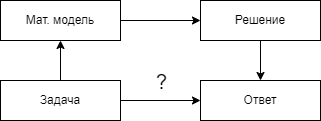
\includegraphics[width=0.65\linewidth]{матмоделизадачи.png}
\end{center}

Основа теории вероятностей - азартные игры (в процессе игры поднимаются ставки).

\section{Парадокс при игре в кости}

Правильная игральная кость при бросании с равными шансами падает на любую из граней 1, 2, 3, 4, 5, 6. 

В случае бросания двух костей сумма выпавших чисел заключена между 2 и 12. 
Как 9, так и 10 из чисел 1, 2, ..., 6 можно получить двумя разными способами: 9=3+6 или 9=4+5 и 10=4+6 или 10=5+5. 
Почему 9 появляется чаще, когда бросают две кости, чем 10?

\textbf{Решение:} 9: 3+6, 6+3, 4+5, 5+4 = 4 из 36 случаев, а 10: 4+6, 6+4, 5+5 = 3 из 36 случаев.

Получается, что 9 выпадает чаще, чем 10, ч.т.д.

\section{Парадокс раздела ставки}

Два игрока играют в безобидную игру (то есть шансы на выигрыш одинаковы) и они договорились, что тот, кто первым выиграет 6 партий, получит весь приз. Предположим, что на самом деле игра остановилась, до того, как один из них выиграл приз (например, первый игрок выиграл 5 партий, второй - 3). Как справедливо следует разделить приз?

\textbf{Решение:} Мысленно представим, что матч бы продолжился. Всего возможно четыре исхода: 
\begin{itemize}
    \item А - 1-ый игрок выигрывает первую партию;
    \item Б - 1-ый игрок выигрывает вторую партию, проиграв первую;
    \item В - 1-ый выигрывает третью, проиграв первую и вторую;
    \item Г - 1-ый проигрывает все партии.
\end{itemize}

Вероятность (\textit{по теореме о независимых событиях}) событий А, Б, В, Г соответственно 0.5, 0.25, 0.125, 0.125 (в сумме 1). 

(*) Вероятность победы 1-го, в таком случае, 0.875, второго - 0.125, то есть в 7 раз меньше. Делим приз на 8 частей - 7 первому, 1 второму.

Ответ: 7:1

\end{document}
